\chapter{减数分裂与遗传重组}\label{ch:g12:meiosis-genetic-shuffling}

双亲各含 46 条\omterm{def:g11:cell-cycle-mitosis:chromosome}{染色体}，却产生含 46 条\omterm{def:g11:cell-cycle-mitosis:chromosome}{染色体}的子代 ——
而非 92 条。在双亲身体与子代之间的某个环节，\omterm{def:g11:cell-cycle-mitosis:chromosome}{染色体}数目
减半，而且减半的方式为每个子代发了一手牌，
这手牌是任何兄弟姐妹都未曾拿过的：同样的双亲，四十年间的子女，
没有两人相同（同卵双胞胎除外）。减半由一种特殊的分裂完成，
称为\omterm{def:g12:meiosis-genetic-shuffling:meiosis}{减数分裂}；“发牌”则是它在分裂过程中对\omterm{def:g11:cell-cycle-mitosis:chromosome}{染色体}所做的
事情。本章追踪一个\omterm{def:g10:cells-common-unit:cell}{细胞}经历\omterm{def:g12:meiosis-genetic-shuffling:meiosis}{减数分裂}的过程，
计算它能产生的组合数，并分析杂交的结果，
这些结果从外部揭示了内部所发生的一切。

\section{染色体数目减半}

\begin{definition}[二倍体、单倍体、减数分裂]\label{def:g12:meiosis-genetic-shuffling:meiosis}
每种\omterm{def:g11:cell-cycle-mitosis:chromosome}{染色体}各有两份的\omterm{def:g10:cells-common-unit:cell}{细胞} ——一份来自父方，一份来自母方，
二者构成一对\emph{\omterm{def:g10:common-ancestry:homology}{同源}\omterm{def:g11:cell-cycle-mitosis:chromosome}{染色体}} ——是
\emph{二倍体}\index{二倍体}，记作 $2n$（人类中 $2n = 46$）。
每种\omterm{def:g11:cell-cycle-mitosis:chromosome}{染色体}仅有一份的\omterm{def:g10:cells-common-unit:cell}{细胞}，称为\emph{单倍体}\index{单倍体}，
记作 $n$。\emph{减数分裂}\index{减数分裂}是连续进行的两次
分裂，一个二倍体\omterm{def:g10:cells-common-unit:cell}{细胞}的 \omterm{def:g10:universal-dna:information}{DNA} 复制一次之后，经此产生
四个单倍体\omterm{def:g10:cells-common-unit:cell}{细胞} ——即配子，或其前体。
\emph{受精}使两个单倍体配子结合，恢复二倍体数目：
减数分裂与受精的交替，是每种有性生殖\omterm{def:g10:biodiversity-scales:species}{物种}的
循环。
\end{definition}

\begin{proposition}[两次分裂]\label{prop:g12:meiosis-genetic-shuffling:divisions}
\omterm{def:g12:meiosis-genetic-shuffling:meiosis}{减数分裂}前 \omterm{def:g10:universal-dna:information}{DNA} 先复制，每条\omterm{def:g11:cell-cycle-mitosis:chromosome}{染色体}含有两条
\omterm{def:g11:cell-cycle-mitosis:chromosome}{染色单体}。之后：
\begin{itemize}
  \item \emph{第一次分裂}（减数第一次分裂，\emph{减数性}）：\omterm{def:g10:common-ancestry:homology}{同源}
        \omterm{def:g11:cell-cycle-mitosis:chromosome}{染色体}两两配对，排列在赤道板上；
        每对中的两条分别被拉向相反的两极。每个
        子\omterm{def:g10:cells-common-unit:cell}{细胞}获得\emph{每对中的一条\omterm{def:g11:cell-cycle-mitosis:chromosome}{染色体}}，
        仍由两条\omterm{def:g11:cell-cycle-mitosis:chromosome}{染色单体}构成：$n$ 条\omterm{def:g11:cell-cycle-mitosis:chromosome}{染色体}，\omterm{def:g10:universal-dna:information}{DNA} 含量 $q$（
        即复制前\omterm{def:g12:meiosis-genetic-shuffling:meiosis}{二倍体}\omterm{def:g10:cells-common-unit:cell}{细胞}的含量）。
  \item \emph{第二次分裂}（减数第二次分裂，\emph{等数性}）：与
        \omterm{def:g11:cell-cycle-mitosis:cycle}{有丝分裂}相似，每条\omterm{def:g11:cell-cycle-mitosis:chromosome}{染色体}的\omterm{def:g11:cell-cycle-mitosis:chromosome}{染色单体}彼此分离。四个\omterm{def:g10:cells-common-unit:cell}{细胞}中的每一个
        获得 $n$ 条仅含一条\omterm{def:g11:cell-cycle-mitosis:chromosome}{染色单体}的\omterm{def:g11:cell-cycle-mitosis:chromosome}{染色体}，
        \omterm{def:g10:universal-dna:information}{DNA} 含量为 $q/2$。
\end{itemize}
第一次分裂使\omterm{def:g11:cell-cycle-mitosis:chromosome}{染色体}数目减半；第二次
分裂使 \omterm{def:g10:universal-dna:information}{DNA} 含量减半，恢复为每条\omterm{def:g11:cell-cycle-mitosis:chromosome}{染色体}一条\omterm{def:g11:cell-cycle-mitosis:chromosome}{染色单体}。
\end{proposition}
\admitted

\begin{omfigure}
\begin{tikzpicture}[font=\small, line cap=round]
  \tikzset{cellb/.style={draw, thick, fill=omDef!5, rounded corners=9pt, minimum width=2.5cm, minimum height=2.5cm},
           ma/.style={line width=3pt, omDef!80}, mb/.style={line width=3pt, omThm!80},
           mA/.style={line width=3pt, omDef!35}, mB/.style={line width=3pt, omThm!35}, cen/.style={fill=black}}
  % panel 1: diploid cell after S: two pairs (long pair blue, short pair red); paternal dark, maternal pale
  \begin{scope}
    \node[cellb] at (0,0) {};
    \draw[ma] (-0.75,0.7) .. controls (-0.62,0.1) .. (-0.75,-0.5); \draw[ma] (-0.49,0.7) .. controls (-0.62,0.1) .. (-0.49,-0.5); \fill[cen] (-0.62,0.1) circle (1.6pt);
    \draw[mA] (-0.2,0.7) .. controls (-0.07,0.1) .. (-0.2,-0.5); \draw[mA] (0.06,0.7) .. controls (-0.07,0.1) .. (0.06,-0.5); \fill[cen] (-0.07,0.1) circle (1.6pt);
    \draw[mb] (0.4,0.45) .. controls (0.53,0.1) .. (0.4,-0.25); \draw[mb] (0.66,0.45) .. controls (0.53,0.1) .. (0.66,-0.25); \fill[cen] (0.53,0.1) circle (1.6pt);
    \draw[mB] (0.9,0.45) .. controls (1.03,0.1) .. (0.9,-0.25); \draw[mB] (1.16,0.45) .. controls (1.03,0.1) .. (1.16,-0.25); \fill[cen] (1.03,0.1) circle (1.6pt);
    \node[anchor=north, align=center, font=\scriptsize, text width=3.05cm] at (0,-1.35) {复制后：\\ $2n = 4$，DNA $2q$};
  \end{scope}
  % panel 2: metaphase I: pairs on the equator
  \begin{scope}[xshift=3.2cm]
    \node[cellb] at (0,0) {};
    \draw[dashed, gray] (-1.1,0) -- (1.1,0);
    \draw[ma] (-0.7,0.55) .. controls (-0.57,0.1) .. (-0.7,-0.35); \draw[ma] (-0.44,0.55) .. controls (-0.57,0.1) .. (-0.44,-0.35); \fill[cen] (-0.57,0.15) circle (1.6pt);
    \draw[mA] (-0.7,-0.05) .. controls (-0.57,-0.5) .. (-0.7,-0.95); \draw[mA] (-0.44,-0.05) .. controls (-0.57,-0.5) .. (-0.44,-0.95); \fill[cen] (-0.57,-0.15) circle (1.6pt);
    \draw[mb] (0.45,0.5) .. controls (0.58,0.2) .. (0.45,-0.1); \draw[mb] (0.71,0.5) .. controls (0.58,0.2) .. (0.71,-0.1); \fill[cen] (0.58,0.15) circle (1.6pt);
    \draw[mB] (0.45,0.1) .. controls (0.58,-0.2) .. (0.45,-0.5); \draw[mB] (0.71,0.1) .. controls (0.58,-0.2) .. (0.71,-0.5); \fill[cen] (0.58,-0.15) circle (1.6pt);
    \node[anchor=north, align=center, font=\scriptsize, text width=3.05cm] at (0,-1.35) {减数第一次分裂：同源 \\ 染色体排列在赤道板上};
  \end{scope}
  % panel 3: two cells after MI, each n=2 with two chromatids
  \begin{scope}[xshift=6.4cm]
    \node[cellb, minimum height=1.15cm] at (0,0.7) {};
    \node[cellb, minimum height=1.15cm] at (0,-0.7) {};
    \draw[ma] (-0.55,1.15) .. controls (-0.42,0.7) .. (-0.55,0.25); \draw[ma] (-0.29,1.15) .. controls (-0.42,0.7) .. (-0.29,0.25); \fill[cen] (-0.42,0.7) circle (1.6pt);
    \draw[mB] (0.35,1.0) .. controls (0.48,0.7) .. (0.35,0.4); \draw[mB] (0.61,1.0) .. controls (0.48,0.7) .. (0.61,0.4); \fill[cen] (0.48,0.7) circle (1.6pt);
    \draw[mA] (-0.55,-0.25) .. controls (-0.42,-0.7) .. (-0.55,-1.15); \draw[mA] (-0.29,-0.25) .. controls (-0.42,-0.7) .. (-0.29,-1.15); \fill[cen] (-0.42,-0.7) circle (1.6pt);
    \draw[mb] (0.35,-0.4) .. controls (0.48,-0.7) .. (0.35,-1.0); \draw[mb] (0.61,-0.4) .. controls (0.48,-0.7) .. (0.61,-1.0); \fill[cen] (0.48,-0.7) circle (1.6pt);
    \node[anchor=north, align=center, font=\scriptsize, text width=3.05cm] at (0,-1.35) {两个细胞：$n = 2$，\\ 每条染色体含两条染色单体，DNA $q$};
  \end{scope}
  % panel 4: four cells after MII, single chromatids
  \begin{scope}[xshift=9.6cm]
    \foreach \y in {1.05,0.35,-0.35,-1.05} \node[cellb, minimum height=0.6cm, minimum width=2.3cm] at (0,\y) {};
    \draw[ma] (-0.5,1.3) -- (-0.5,0.8); \fill[cen] (-0.5,1.05) circle (1.4pt); \draw[mB] (0.4,1.22) -- (0.4,0.88); \fill[cen] (0.4,1.05) circle (1.4pt);
    \draw[ma] (-0.5,0.6) -- (-0.5,0.1); \fill[cen] (-0.5,0.35) circle (1.4pt); \draw[mB] (0.4,0.52) -- (0.4,0.18); \fill[cen] (0.4,0.35) circle (1.4pt);
    \draw[mA] (-0.5,-0.1) -- (-0.5,-0.6); \fill[cen] (-0.5,-0.35) circle (1.4pt); \draw[mb] (0.4,-0.18) -- (0.4,-0.52); \fill[cen] (0.4,-0.35) circle (1.4pt);
    \draw[mA] (-0.5,-0.8) -- (-0.5,-1.3); \fill[cen] (-0.5,-1.05) circle (1.4pt); \draw[mb] (0.4,-0.88) -- (0.4,-1.22); \fill[cen] (0.4,-1.05) circle (1.4pt);
    \node[anchor=north, align=center, font=\scriptsize, text width=3.05cm] at (0,-1.45) {四个配子：$n = 2$，\\ 每条染色体含一条染色单体，DNA $q/2$};
  \end{scope}
\end{tikzpicture}

{\small 含两对\omterm{def:g11:cell-cycle-mitosis:chromosome}{染色体}（$2n = 4$）的\omterm{def:g10:cells-common-unit:cell}{细胞}中的\omterm{def:g12:meiosis-genetic-shuffling:meiosis}{减数分裂}；
深色与浅色分别标示每对中来自两个
亲本的两条\omterm{def:g11:cell-cycle-mitosis:chromosome}{染色体}。第一次分裂分离\omterm{def:g10:common-ancestry:homology}{同源}\omterm{def:g11:cell-cycle-mitosis:chromosome}{染色体}，第二次分裂分离
\omterm{def:g11:cell-cycle-mitosis:chromosome}{染色单体}。此处深色长\omterm{def:g11:cell-cycle-mitosis:chromosome}{染色体}与浅色短\omterm{def:g11:cell-cycle-mitosis:chromosome}{染色体}进入了同一个子\omterm{def:g10:cells-common-unit:cell}{细胞}：
两种可能组合之一。}
\end{omfigure}

\begin{omfigure}
\begin{tikzpicture}
\begin{axis}[
  width=0.88\linewidth, height=5.2cm,
  axis x line=bottom, axis y line=left,
  xmin=0, xmax=10, ymin=0, ymax=2.7,
  xlabel={时间}, ylabel={每个细胞的 DNA 含量},
  xlabel style={font=\small, at={(axis description cs:0.5,-0.1)}, anchor=north},
  ylabel style={font=\small},
  tick label style={font=\small}, xtick=\empty,
  ytick={0.5,1,2}, yticklabels={$q/2$, $q$, $2q$},
  clip=false,
]
\addplot[thick, omDef] coordinates {(0,1) (2,1) (4,2) (5.9,2) (6,1) (7.9,1) (8,0.5) (10,0.5)};
\draw[dashed, gray] (axis cs:2,0) -- (axis cs:2,2.2); \draw[dashed, gray] (axis cs:4,0) -- (axis cs:4,2.2);
\draw[dashed, gray] (axis cs:6,0) -- (axis cs:6,2.2); \draw[dashed, gray] (axis cs:8,0) -- (axis cs:8,2.2);
\node[font=\small, anchor=south] at (axis cs:1,2.25) {$2n$, $q$};
\node[font=\small, anchor=south] at (axis cs:3,2.25) {S 期};
\node[font=\small, anchor=south] at (axis cs:5,2.25) {$2n$, $2q$};
\node[font=\small, anchor=south, omThm] at (axis cs:6,2.45) {减数第一次分裂};
\node[font=\small, anchor=south] at (axis cs:7,2.25) {$n$, $q$};
\node[font=\small, anchor=south, omThm] at (axis cs:8,2.45) {减数第二次分裂};
\node[font=\small, anchor=south] at (axis cs:9,2.25) {$n$, $q/2$};
\end{axis}
\end{tikzpicture}

{\small \omterm{def:g12:meiosis-genetic-shuffling:meiosis}{减数分裂}中每个\omterm{def:g10:cells-common-unit:cell}{细胞}的 \omterm{def:g10:universal-dna:information}{DNA} 量。先复制一次，然后连续两次分裂，
两次分裂之间不再复制：配子所含的 \omterm{def:g10:universal-dna:information}{DNA} 量，
为母\omterm{def:g10:cells-common-unit:cell}{细胞}在 S 期后所含的四分之一，
也是\omterm{def:g12:meiosis-genetic-shuffling:meiosis}{二倍体}\omterm{def:g10:cells-common-unit:cell}{细胞}静止时所含的一半。}
\end{omfigure}

\begin{example}[人类的数目]\label{ex:g12:meiosis-genetic-shuffling:numbers}
睾丸中的一个生殖\omterm{def:g10:cells-common-unit:cell}{细胞}，$2n = 46$，复制后形成 46 条含两条\omterm{def:g11:cell-cycle-mitosis:chromosome}{染色单体}的
\omterm{def:g11:cell-cycle-mitosis:chromosome}{染色体}（$2q$）；减数第一次分裂后形成两个\omterm{def:g10:cells-common-unit:cell}{细胞}，各含 23 条含两条\omterm{def:g11:cell-cycle-mitosis:chromosome}{染色单体}的
\omterm{def:g11:cell-cycle-mitosis:chromosome}{染色体}（$q$）；减数第二次分裂后形成四个精子\omterm{def:g10:cells-common-unit:cell}{细胞}，各含 23 条
含单条\omterm{def:g11:cell-cycle-mitosis:chromosome}{染色单体}的\omterm{def:g11:cell-cycle-mitosis:chromosome}{染色体}（$q/2$）。受精时，$23 + 23 =
46$，$q/2 + q/2 = q$：受精卵重新成为静止的\omterm{def:g12:meiosis-genetic-shuffling:meiosis}{二倍体}\omterm{def:g10:cells-common-unit:cell}{细胞}。
在卵巢中，同样的分裂产生一个大卵\omterm{def:g10:cells-common-unit:cell}{细胞}和三个
微小的、会被舍弃的\omterm{def:g10:cells-common-unit:cell}{细胞}；计算过程完全相同。
\end{example}

\section{混合}

\begin{proposition}[自由组合]\label{prop:g12:meiosis-genetic-shuffling:assortment}
在减数第一次分裂中期，每一对\omterm{def:g10:common-ancestry:homology}{同源}\omterm{def:g11:cell-cycle-mitosis:chromosome}{染色体}
在赤道板上排列，彼此独立：每对\omterm{def:g11:cell-cycle-mitosis:chromosome}{染色体}中哪一条
移向哪一极由偶然决定，逐对独立进行。因此，含 $n$ 对的\omterm{def:g10:cells-common-unit:cell}{细胞}
可在配子中产生 $2^n$ 种不同的父源与母源\omterm{def:g11:cell-cycle-mitosis:chromosome}{染色体}组合
——人类中为 $2^{23} \approx \num{8.4e6}$ 种。
受精时两个这样的配子随机结合，产生 $2^{23}
\times 2^{23} \approx \num{7e13}$ 种\omterm{def:g11:cell-cycle-mitosis:chromosome}{染色体}组合，即一对夫妇的子女
可能具有的组合，尚未计入其他变异来源。
\end{proposition}
\admitted

\begin{proposition}[交叉互换]\label{prop:g12:meiosis-genetic-shuffling:crossingover}
在减数第一次分裂前期，\omterm{def:g10:common-ancestry:homology}{同源}\omterm{def:g11:cell-cycle-mitosis:chromosome}{染色体}配对时，两条非姐妹
\omterm{def:g11:cell-cycle-mitosis:chromosome}{染色单体}在同一位点断裂并交叉重接，这称为
\emph{交叉互换}\index{交叉互换}。交换点之外的每条\omterm{def:g11:cell-cycle-mitosis:chromosome}{染色单体}
现在携带另一条\omterm{def:g10:common-ancestry:homology}{同源}\omterm{def:g11:cell-cycle-mitosis:chromosome}{染色体}的\omterm{def:g10:universal-dna:gene}{等位基因}。因此，进入配子的
\omterm{def:g11:cell-cycle-mitosis:chromosome}{染色体}不再是亲代的\omterm{def:g11:cell-cycle-mitosis:chromosome}{染色体}，而是\emph{重组}\omterm{def:g11:cell-cycle-mitosis:chromosome}{染色体}，
沿其长度混合了来自两个祖代的\omterm{def:g10:universal-dna:gene}{等位基因}。每对\omterm{def:g11:cell-cycle-mitosis:chromosome}{染色体}在每次
\omterm{def:g12:meiosis-genetic-shuffling:meiosis}{减数分裂}中都发生一至三次交换，位置各不相同，
配子的可能种类
实际上不可胜数。
\end{proposition}
\begin{proof}[证据]
在显微镜下，减数第一次分裂中配对的\omterm{def:g10:common-ancestry:homology}{同源}\omterm{def:g11:cell-cycle-mitosis:chromosome}{染色体}显示出交叉点，
\emph{交叉点}，两条\omterm{def:g11:cell-cycle-mitosis:chromosome}{染色单体}在此可见地相互交换。
若两个\omterm{def:g10:universal-dna:gene}{基因}位于同一\omterm{def:g11:cell-cycle-mitosis:chromosome}{染色体}上，
其杂交后代中有少数个体带有两个\omterm{def:g10:universal-dna:gene}{基因}\omterm{def:g10:universal-dna:gene}{等位基因}的新组合，
即亲本都不具有的组合——其比例
取决于两个\omterm{def:g10:universal-dna:gene}{基因}之间的距离；位于同一\omterm{def:g11:cell-cycle-mitosis:chromosome}{染色体}上相距较远的\omterm{def:g10:universal-dna:gene}{基因}
重组的频率与位于不同\omterm{def:g11:cell-cycle-mitosis:chromosome}{染色体}上的\omterm{def:g10:universal-dna:gene}{基因}相同。
通过家系追踪的分子标记表明，每条\omterm{def:g11:cell-cycle-mitosis:chromosome}{染色体}的各个片段
在祖代来源之间切换，每代每条\omterm{def:g11:cell-cycle-mitosis:chromosome}{染色体}上
约有一至两处切换点。
\end{proof}

\begin{omfigure}
\begin{tikzpicture}[font=\small, line cap=round, >=Stealth]
  \tikzset{p/.style={line width=4pt, omDef!80}, m/.style={line width=4pt, omThm!70}}
  % before: two homologues, each two chromatids; alleles A/a, B/b
  \draw[p] (0,0) -- (0,3); \draw[p] (0.35,0) -- (0.35,3);
  \draw[m] (0.9,0) -- (0.9,3); \draw[m] (1.25,0) -- (1.25,3);
  \foreach \x in {0,0.35} { \node[font=\scriptsize, anchor=east, xshift=-1pt] at (\x,2.6) {}; }
  \node[font=\scriptsize, omDef!80!black, anchor=east] at (-0.15,2.6) {$A$};
  \node[font=\scriptsize, omDef!80!black, anchor=east] at (-0.15,0.5) {$B$};
  \node[font=\scriptsize, omThm!80!black, anchor=west] at (1.4,2.6) {$a$};
  \node[font=\scriptsize, omThm!80!black, anchor=west] at (1.4,0.5) {$b$};
  \node[anchor=north, align=center] at (0.62,-0.2) {配对的同源染色体 \\（各含两条染色单体）};
  \draw[->, thick] (2.4,1.5) -- (3.4,1.5);
  % during: chiasma between the two inner chromatids at y=1.5
  \begin{scope}[xshift=4.2cm]
    \draw[p] (0,0) -- (0,3);
    \draw[p] (0.35,3) -- (0.35,1.6) -- (0.9,1.4) -- (0.9,0);
    \draw[m] (0.9,3) -- (0.9,1.6) -- (0.35,1.4) -- (0.35,0);
    \draw[m] (1.25,0) -- (1.25,3);
    \node[anchor=north, align=center] at (0.62,-0.2) {交叉点：两条染色单体 \\ 断裂后交叉重接};
  \end{scope}
  \draw[->, thick] (6.6,1.5) -- (7.6,1.5);
  % after: four chromatids separated
  \begin{scope}[xshift=8.4cm]
    \draw[p] (0,0) -- (0,3);
    \draw[p] (0.5,3) -- (0.5,1.5); \draw[m] (0.5,1.5) -- (0.5,0);
    \draw[m] (1.0,3) -- (1.0,1.5); \draw[p] (1.0,1.5) -- (1.0,0);
    \draw[m] (1.5,0) -- (1.5,3);
    \node[font=\scriptsize, anchor=south] at (0,3.05) {$AB$};
    \node[font=\scriptsize, anchor=south] at (0.5,3.05) {$Ab$};
    \node[font=\scriptsize, anchor=south] at (1.0,3.05) {$aB$};
    \node[font=\scriptsize, anchor=south] at (1.5,3.05) {$ab$};
    \node[anchor=north, align=center] at (0.75,-0.2) {四个配子：两个亲本型，\\ 两个重组型};
  \end{scope}
\end{tikzpicture}

{\small 同一\omterm{def:g11:cell-cycle-mitosis:chromosome}{染色体}上两个\omterm{def:g10:universal-dna:gene}{基因} $A$ 和 $B$ 之间的\omterm{prop:g12:meiosis-genetic-shuffling:crossingover}{交叉互换}。
四条\omterm{def:g11:cell-cycle-mitosis:chromosome}{染色单体}中有两条交换末端；四个配子中，
两个带有亲本组合（$AB$、$ab$），两个为新组合
（$Ab$、$aB$）。}
\end{omfigure}

\begin{omfigure}
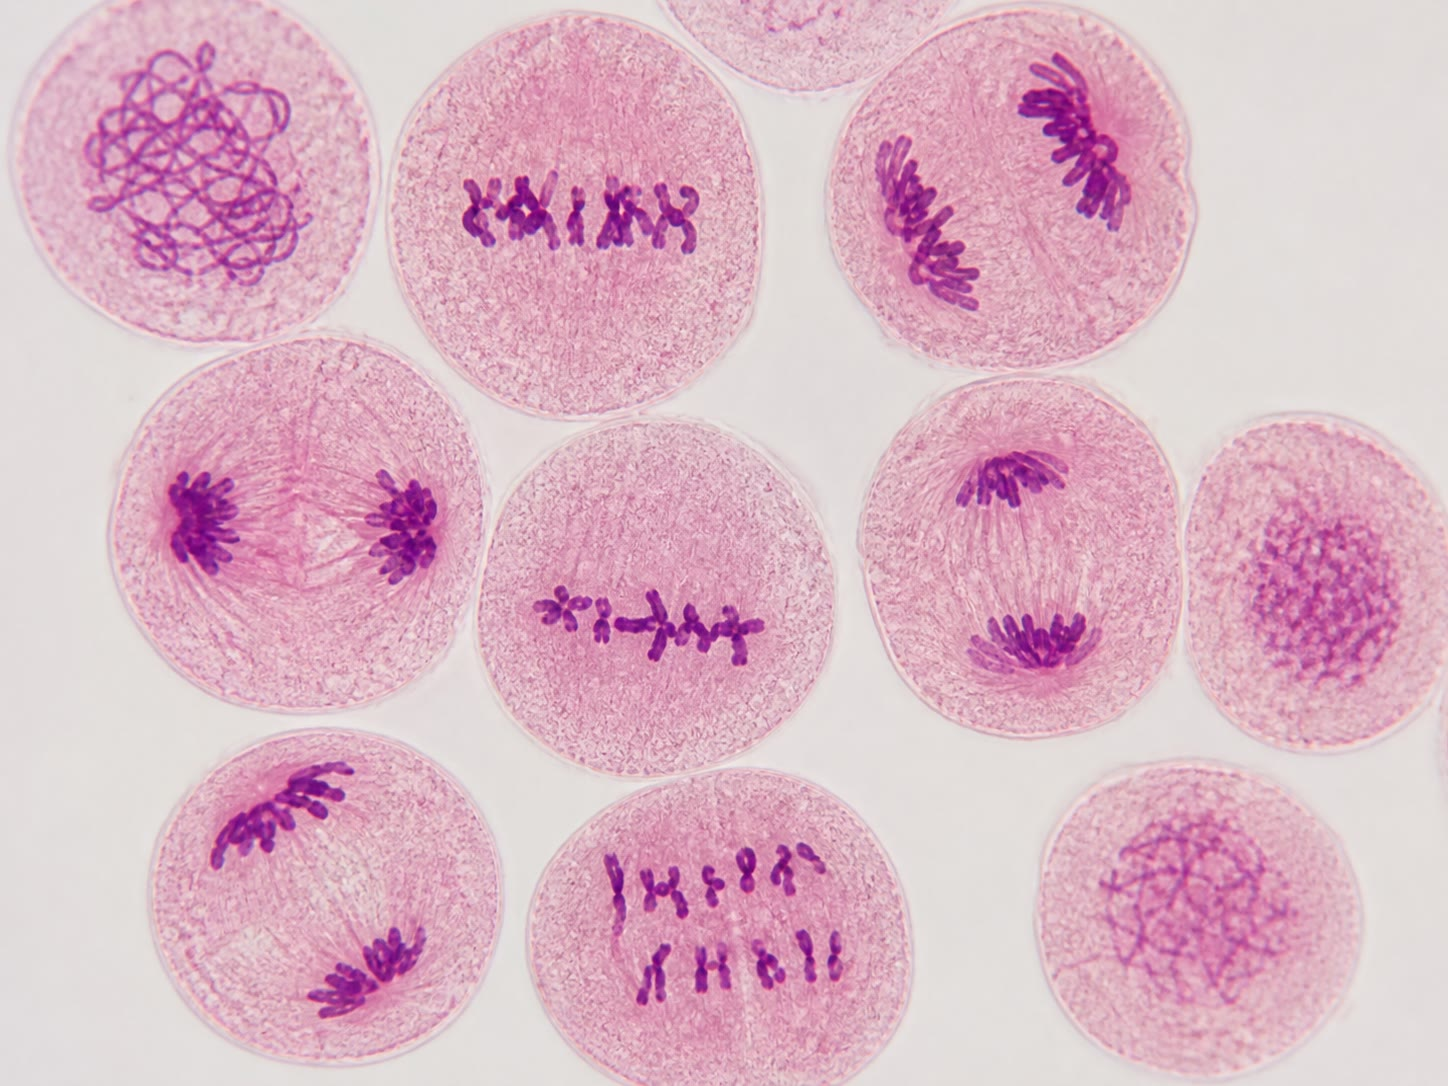
\includegraphics[width=0.56\linewidth]{images/book2/ai/g12-meiosis-lily-anther.jpg}

{\small 百合花药中\omterm{def:g12:meiosis-genetic-shuffling:meiosis}{减数分裂}的\omterm{def:g10:cells-common-unit:cell}{细胞}，经染色：有些\omterm{def:g10:cells-common-unit:cell}{细胞}中，
配对的\omterm{def:g10:common-ancestry:homology}{同源}\omterm{def:g11:cell-cycle-mitosis:chromosome}{染色体}排列在\omterm{def:g10:cells-common-unit:cell}{细胞}中部；另一些中，
\omterm{def:g10:common-ancestry:homology}{同源}\omterm{def:g11:cell-cycle-mitosis:chromosome}{染色体}已被拉向两极。示意图的各阶段，
均见于产生花粉的组织。}
\end{omfigure}

\begin{example}[变异的三个来源，依次列出]\label{ex:g12:meiosis-genetic-shuffling:sources}
双亲的子女在三个方面是全新的：\omterm{prop:g12:meiosis-genetic-shuffling:crossingover}{交叉互换}由两个祖代拷贝
重新组建了每个配子中的每条\omterm{def:g11:cell-cycle-mitosis:chromosome}{染色体}；
自由组合在每对\omterm{def:g11:cell-cycle-mitosis:chromosome}{染色体}中各选出一条重组\omterm{def:g11:cell-cycle-mitosis:chromosome}{染色体}
放入配子，共有 $2^{23}$ 种分配方式；受精则使一个这样的
配子与另一亲本 $2^{23}$ 种配子中抽出的一个结合。\omterm{def:g11:mutations:mutation}{突变}
产生了被混合的\omterm{def:g10:universal-dna:gene}{等位基因}，但其作用的时间尺度慢得多：
正是混合，使每一代都能从同一副牌中
发出全新的组合。
\end{example}

\section{解读杂交中的混合}

\begin{omfigure}
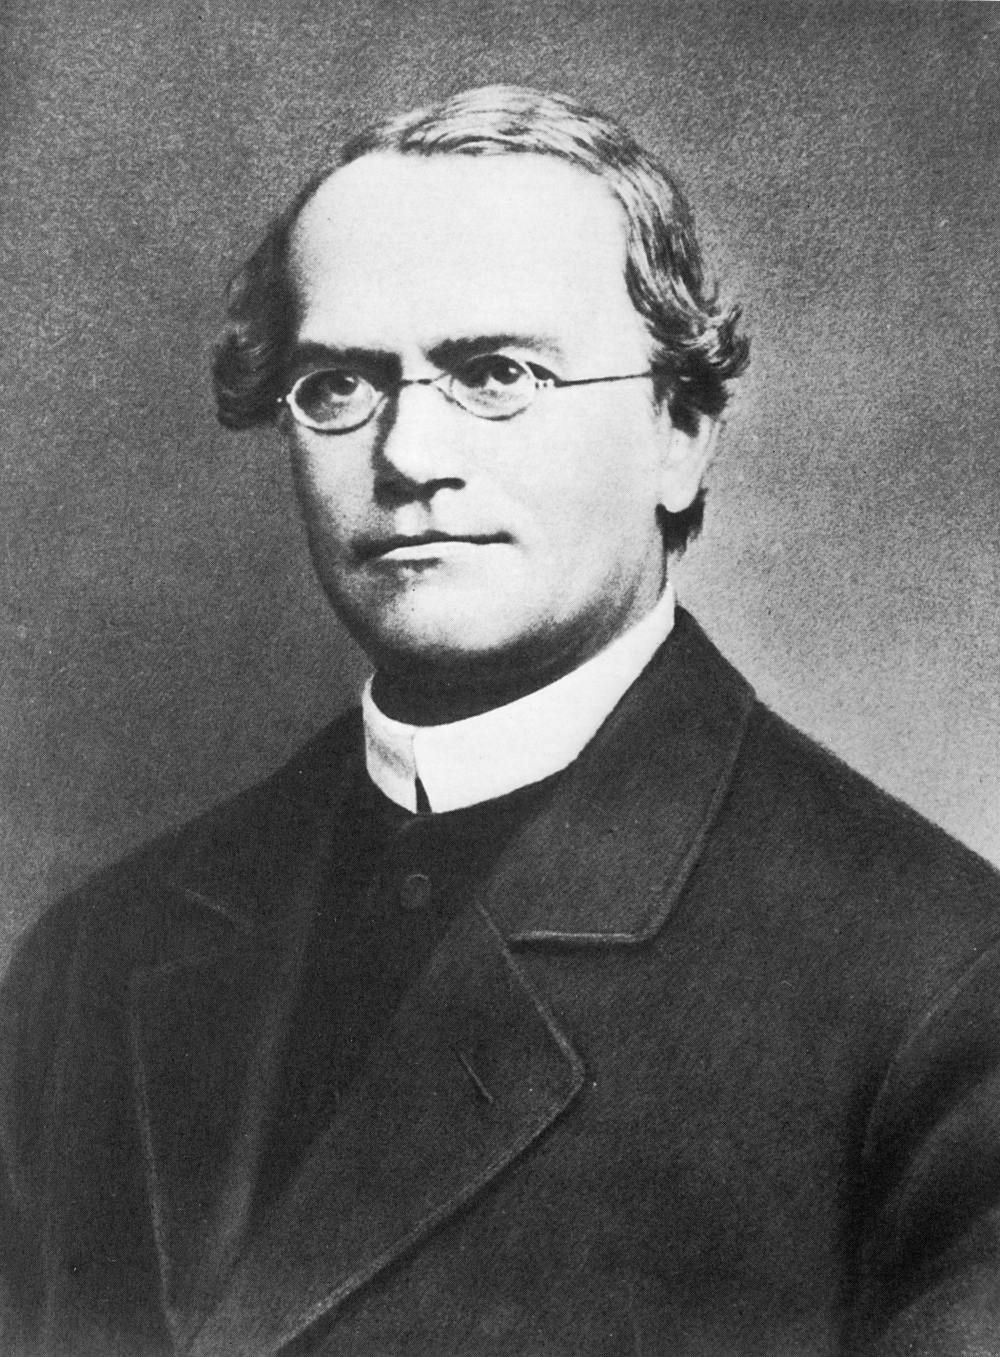
\includegraphics[width=0.3\linewidth]{images/book2/mendel.jpg}

{\small 格雷戈尔·孟德尔在 1860 年代于修道院花园中统计豌豆杂交的后代，发现了 3:1（一对性状）和 9:3:3:1（两对性状）的比例——这正是他并不知道的\omterm{def:g12:meiosis-genetic-shuffling:meiosis}{减数分裂}所产生的比例。照片，公有领域。}
\end{omfigure}

\begin{method}[测交]\label{met:g12:meiosis-genetic-shuffling:testcross}
要看一个个体能产生哪些配子，可将它与只带\omterm{def:g11:genes-and-disease:genetic}{隐性}\omterm{def:g10:universal-dna:gene}{等位基因}的个体杂交
（称为\emph{测交}）：每个子代
都恰好显示出被测亲本配子所携带的\omterm{def:g10:universal-dna:gene}{等位基因}。
对于两个\omterm{def:g10:universal-dna:gene}{基因}，设被测亲本为 $AaBb$，另一亲本为 $aabb$：
\begin{enumerate}
  \item 数出子代的四种类型：$AB$、$Ab$、$aB$、$ab$
        （每一类均另含来自另一亲本的 $ab$）
  \item 若四类个体数相等（$1:1:1:1$），则两\omterm{def:g10:universal-dna:gene}{基因}位于
        不同\omterm{def:g11:cell-cycle-mitosis:chromosome}{染色体}上，自由组合。
  \item 若其中两类（亲本组合）远多于
        另两类（重组类型），则两\omterm{def:g10:universal-dna:gene}{基因}位于同一条
        \omterm{def:g11:cell-cycle-mitosis:chromosome}{染色体}上；重组类型来自\omterm{prop:g12:meiosis-genetic-shuffling:crossingover}{交叉互换}，其
        比例可以度量两\omterm{def:g10:universal-dna:gene}{基因}之间的距离。
  \item 重组类型总是少数，且总是成两个相等的类别出现；
        亲本类型亦然。
\end{enumerate}
\end{method}

\begin{example}[果蝇的两次杂交]\label{ex:g12:meiosis-genetic-shuffling:fly}
果蝇 A 在体色和翅形上为杂合，进行测交，得到子代 254 只灰体正常翅，
248 只黑体残翅，251 只灰体残翅，247 只
黑体正常翅——四类数目相等，两\omterm{def:g10:universal-dna:gene}{基因}位于不同
\omterm{def:g11:cell-cycle-mitosis:chromosome}{染色体}上。果蝇 B 在体色和眼色上为杂合：
灰体红眼 412、黑体紫眼 405、灰体紫眼 44、黑体红眼 39——两类
亲本型各占约 45\%，两类重组型
各占约 5\%：两\omterm{def:g10:universal-dna:gene}{基因}位于同一条\omterm{def:g11:cell-cycle-mitosis:chromosome}{染色体}上，且彼此靠近，
约 9\% 的\omterm{def:g12:meiosis-genetic-shuffling:meiosis}{减数分裂}中发生\omterm{prop:g12:meiosis-genetic-shuffling:crossingover}{交叉互换}，使二者分离。
\end{example}

\begin{omfigure}
\begin{tikzpicture}[font=\small]
  \draw[thick] (0,0) grid[step=1.4] (5.6,1.4);
  \node[fill=omDef!15, minimum width=1.3cm, minimum height=1.3cm, align=center] at (0.7,0.7) {$AB$\\ 254};
  \node[fill=omDef!15, minimum width=1.3cm, minimum height=1.3cm, align=center] at (2.1,0.7) {$Ab$\\ 251};
  \node[fill=omDef!15, minimum width=1.3cm, minimum height=1.3cm, align=center] at (3.5,0.7) {$aB$\\ 247};
  \node[fill=omDef!15, minimum width=1.3cm, minimum height=1.3cm, align=center] at (4.9,0.7) {$ab$\\ 248};
  \node[anchor=south] at (2.8,1.5) {果蝇 A：独立基因，$1:1:1:1$};
  \begin{scope}[xshift=7.4cm]
    \draw[thick] (0,0) grid[step=1.4] (5.6,1.4);
    \node[fill=omProp!25, minimum width=1.3cm, minimum height=1.3cm, align=center] at (0.7,0.7) {$AB$\\ 412};
    \node[fill=omThm!20, minimum width=1.3cm, minimum height=1.3cm, align=center] at (2.1,0.7) {$Ab$\\ 44};
    \node[fill=omThm!20, minimum width=1.3cm, minimum height=1.3cm, align=center] at (3.5,0.7) {$aB$\\ 39};
    \node[fill=omProp!25, minimum width=1.3cm, minimum height=1.3cm, align=center] at (4.9,0.7) {$ab$\\ 405};
    \node[anchor=south] at (2.8,1.5) {果蝇 B：连锁基因，亲本型 $\gg$ 重组型};
  \end{scope}
\end{tikzpicture}

{\small 由测交结果读出两只杂合果蝇的配子。
各类数目相等表示独立分配；两大两小
表示两\omterm{def:g10:universal-dna:gene}{基因}连锁，其中两小类由
\omterm{prop:g12:meiosis-genetic-shuffling:crossingover}{交叉互换}产生。}
\end{omfigure}

\section{混合出错时}

\begin{proposition}[减数分裂的错误]\label{prop:g12:meiosis-genetic-shuffling:errors}
偶尔，一对\omterm{def:g10:common-ancestry:homology}{同源}\omterm{def:g11:cell-cycle-mitosis:chromosome}{染色体}在减数第一次分裂时未能分离，或
两条\omterm{def:g11:cell-cycle-mitosis:chromosome}{染色单体}在减数第二次分裂时未能分离：一个配子得到某条\omterm{def:g11:cell-cycle-mitosis:chromosome}{染色体}的两份拷贝，
另一个配子则一份也没有。受精后，它们形成具有三份拷贝的合子
（\emph{三体}）或仅一份（\emph{单体}）。这类合子大多不能发育；
能发育的则带有一组特征性
表现。21 三体（约每 700 例出生中有一例）导致智力
障碍和心脏缺陷，是最常见的一种；其发生频率
随母亲年龄急剧上升。不等\omterm{prop:g12:meiosis-genetic-shuffling:crossingover}{交叉互换}——
即\omterm{def:g11:cell-cycle-mitosis:chromosome}{染色单体}交换长度不等的片段——产生一条带有
重复\omterm{def:g10:universal-dna:gene}{基因}的\omterm{def:g11:cell-cycle-mitosis:chromosome}{染色体}，另一条则发生缺失：这正是
在\cref{ch:g11:the-eye}中\omterm{def:g11:the-eye:photoreceptors}{视蛋白}\omterm{def:g10:universal-dna:gene}{基因}得以增殖的机制，也是
新\omterm{def:g10:universal-dna:gene}{基因}产生的途径（见\cref{ch:g12:diversification-of-life}）。
\end{proposition}
\admitted

\begin{omfigure}
\begin{tikzpicture}
\begin{axis}[
  width=0.84\linewidth, height=5.4cm,
  axis x line=bottom, axis y line=left,
  xmin=18, xmax=47, ymin=0, ymax=40,
  xlabel={母亲年龄（岁）}, ylabel={每 1000 例出生中的 21 三体数},
  xlabel style={font=\small, at={(axis description cs:0.5,-0.12)}, anchor=north},
  ylabel style={font=\small},
  tick label style={font=\small}, xtick={20,25,30,35,40,45}, ytick={0,10,20,30,40},
]
\addplot[thick, omThm, mark=*, mark size=1.5pt] coordinates
  {(20,0.7) (25,0.8) (30,1.1) (33,1.8) (35,2.9) (37,4.5) (39,7.5) (41,12) (43,20) (45,33)};
\end{axis}
\end{tikzpicture}

{\small 出生时 21 三体的频率与母亲年龄的关系。
卵\omterm{def:g10:cells-common-unit:cell}{细胞}在女性出生前即已形成，并在减数第一次分裂中停滞
数十年；停滞越久，\omterm{def:g10:common-ancestry:homology}{同源}\omterm{def:g11:cell-cycle-mitosis:chromosome}{染色体}
未能分离的可能性就越大。}
\end{omfigure}

\begin{example}[性染色体数目出错]\label{ex:g12:meiosis-genetic-shuffling:sexchrom}
不含\omterm{def:g11:becoming-male-female:chromosomes}{性染色体}的配子与携带 X 的配子受精，
形成 XO 合子：一名身材矮小、卵巢不发育的女孩。
XX 卵\omterm{def:g10:cells-common-unit:cell}{细胞}被携带 Y 的精子受精，形成 XXY 合子：一名
睾丸细小、不产生精子的男孩。两种情况下，\omterm{prop:g11:becoming-male-female:sry}{SRY} 决定性腺的发育方向，
见\cref{ch:g11:becoming-male-female}；X \omterm{def:g11:cell-cycle-mitosis:chromosome}{染色体}的数目
决定了其余的大部分表现，这正是这类错误
在\omterm{def:g11:cell-cycle-mitosis:chromosome}{染色体}错误中最轻微的原因。
\end{example}

\begin{remark}[为何有性]\label{rem:g12:meiosis-genetic-shuffling:whysex}
细菌自行复制；月季可以从插枝长成新株。有性
生殖代价更高——需要双亲、\omterm{def:g12:meiosis-genetic-shuffling:meiosis}{减数分裂}，还要寻找
配偶——，其产物是一组后代，每一个都与亲代
及彼此不同。这种差异正是关键：在
环境不断变化、寄生虫不断演化的情况下，
由各异个体组成的种群，更可能含有一些能存活的个体，
而由复制品组成的种群则不然。本章的重组
正是后两章中自然选择将要筛选的原材料。
\end{remark}

\section{练习}

\begin{exercise}[$\star$]\label{exo:g12:meiosis-genetic-shuffling:1}
定义\omterm{def:g12:meiosis-genetic-shuffling:meiosis}{二倍体}与\omterm{def:g12:meiosis-genetic-shuffling:meiosis}{单倍体}，并说明\omterm{def:g12:meiosis-genetic-shuffling:meiosis}{减数分裂}对
\omterm{def:g11:cell-cycle-mitosis:chromosome}{染色体}数目和 \omterm{def:g10:universal-dna:information}{DNA} 含量有何影响。
\end{exercise}

\begin{exercise}[$\star$]\label{exo:g12:meiosis-genetic-shuffling:2}
减数第一次分裂时哪些成分分开？减数第二次分裂时呢？
哪一次分裂使\omterm{def:g11:cell-cycle-mitosis:chromosome}{染色体}数目减半？
\end{exercise}

\begin{exercise}[$\star$]\label{exo:g12:meiosis-genetic-shuffling:3}
某\omterm{def:g10:cells-common-unit:cell}{细胞}在\omterm{def:g12:meiosis-genetic-shuffling:meiosis}{减数分裂}开始时，\omterm{def:g11:cell-cycle-mitosis:chromosome}{染色体}数目为 $2n = 8$，\omterm{def:g10:universal-dna:information}{DNA} 含量为 $2q$。求
减数第一次分裂后与减数第二次分裂后\omterm{def:g10:cells-common-unit:cell}{细胞}的\omterm{def:g11:cell-cycle-mitosis:chromosome}{染色体}数目和
\omterm{def:g10:universal-dna:information}{DNA} 含量。
\end{exercise}

\begin{exercise}[$\star$]\label{exo:g12:meiosis-genetic-shuffling:4}
仅凭自由组合作用，
\omterm{def:g11:cell-cycle-mitosis:chromosome}{染色体}数目为 $2n = 8$ 的\omterm{def:g10:biodiversity-scales:species}{物种}，其配子能出现多少种\omterm{def:g11:cell-cycle-mitosis:chromosome}{染色体}组合？
\end{exercise}

\begin{exercise}[$\star$]\label{exo:g12:meiosis-genetic-shuffling:5}
什么是测交，测交后代中重组型个体的比例
说明了什么？
\end{exercise}

\begin{exercise}[$\star\star$]\label{exo:g12:meiosis-genetic-shuffling:6}
根据 \omterm{def:g10:universal-dna:information}{DNA} 图，读出减数第一次分裂中的\omterm{def:g10:cells-common-unit:cell}{细胞}、
两次分裂之间的\omterm{def:g10:cells-common-unit:cell}{细胞}以及配子的每\omterm{def:g10:cells-common-unit:cell}{细胞} \omterm{def:g10:universal-dna:information}{DNA} 含量，
并解释为何两次分裂之间没有 S 期。
\end{exercise}

\begin{exercise}[$\star\star$]\label{exo:g12:meiosis-genetic-shuffling:7}
一次测交得到 300 个 $AB$、298 个 $ab$、302 个 $Ab$、300 个 $aB$。两\omterm{def:g10:universal-dna:gene}{基因}
是否连锁？亲本产生的配子分别是什么？
\end{exercise}

\begin{exercise}[$\star\star$]\label{exo:g12:meiosis-genetic-shuffling:8}
一次测交得到 460 个 $AB$、455 个 $ab$、42 个 $Ab$、43 个 $aB$。两\omterm{def:g10:universal-dna:gene}{基因}
是否连锁？哪些类型为重组型？它们占多大比例？
\end{exercise}

\begin{exercise}[$\star\star$]\label{exo:g12:meiosis-genetic-shuffling:9}
在\omterm{prop:g12:meiosis-genetic-shuffling:crossingover}{交叉互换}图中，若交换发生在
两个\omterm{def:g10:universal-dna:gene}{基因}的\emph{上方}，会得到哪两种配子？请解释。
\end{exercise}

\begin{exercise}[$\star\star$]\label{exo:g12:meiosis-genetic-shuffling:10}
根据三体图，读出 25、35 和 42 岁时的频率，
并计算 25 岁与 42 岁之间的倍数。
\end{exercise}

\begin{exercise}[$\star\star$]\label{exo:g12:meiosis-genetic-shuffling:11}
请解释减数第一次分裂的不分离与减数第二次分裂的不分离
在所产生的配子上有何不同（考虑全部四个\omterm{def:g10:cells-common-unit:cell}{细胞}）。
\end{exercise}

\begin{exercise}[$\star\star\star$]\label{exo:g12:meiosis-genetic-shuffling:12}
位于同一条\omterm{def:g11:cell-cycle-mitosis:chromosome}{染色体}上的两个\omterm{def:g10:universal-dna:gene}{基因}在 2\% 的\omterm{def:g12:meiosis-genetic-shuffling:meiosis}{减数分裂}中发生重组；
同一条\omterm{def:g11:cell-cycle-mitosis:chromosome}{染色体}上的另外两个\omterm{def:g10:universal-dna:gene}{基因}则在 48\% 的\omterm{def:g12:meiosis-genetic-shuffling:meiosis}{减数分裂}中发生重组。请解释这两个数字
分别说明了它们之间的距离，以及为何第二对\omterm{def:g10:universal-dna:gene}{基因}的行为几乎
与独立遗传的\omterm{def:g10:universal-dna:gene}{基因}相似。
\end{exercise}

\begin{exercise}[$\star\star\star$]\label{exo:g12:meiosis-genetic-shuffling:13}
一株植物 $2n = 4$，其中一对携带 $A/a$，另一对携带 $B/b$。
列出 $AaBb$ 植株的全部配子及其频率，
假设不发生\omterm{prop:g12:meiosis-genetic-shuffling:crossingover}{交叉互换}；然后说明\omterm{prop:g12:meiosis-genetic-shuffling:crossingover}{交叉互换}会改变什么。
\end{exercise}

\begin{exercise}[$\star\star\star$]\label{exo:g12:meiosis-genetic-shuffling:14}
同卵双胞胎共享全部\omterm{def:g10:universal-dna:gene}{等位基因}；普通兄弟姐妹
平均共享一半。请结合\omterm{def:g12:meiosis-genetic-shuffling:meiosis}{减数分裂}与受精解释这“一半”，以及
它为何是一个平均值。
\end{exercise}

\begin{exercise}[$\star\star\star$]\label{exo:g12:meiosis-genetic-shuffling:15}
有些植物的种子不经\omterm{def:g12:meiosis-genetic-shuffling:meiosis}{减数分裂}和
受精即可形成，它们以此繁殖。请解释这类后代在遗传上是什么情况，这种植物
获得了什么，长远看又失去了什么。
\end{exercise}

\section{问题：遗传学家的果蝇}

\begin{problem}[{周末问题——追踪两个基因经过减数分裂与测交的过程：
统计配子、判定连锁、
测定重组率，以及一对夫妇能“发出”的手数}]
\label{pb:g12:meiosis-genetic-shuffling:1}
在果蝇中，\omterm{def:g10:universal-dna:gene}{等位基因} $b$（黑身）对 $b^+$
（灰身）为\omterm{def:g11:genes-and-disease:genetic}{隐性}，$vg$（残翅）对 $vg^+$（正常翅）为\omterm{def:g11:genes-and-disease:genetic}{隐性}。一只
灰身、正常翅的雌果蝇，其亲本分别为纯合灰身正常翅与
纯合黑身残翅，该雌果蝇与一只黑身残翅的雄果蝇杂交，后代为：
灰身正常翅 965 只、黑身残翅 944 只、灰身残翅 206 只、黑身正常翅
185 只。

\medskip
\noindent\textbf{第一部分——杂交。}
\begin{enumerate}
  \item 按\omterm{def:g10:universal-dna:gene}{基因}逐一写出雌果蝇和雄果蝇的\omterm{def:g11:enzymes-and-phenotype:phenotype}{基因型}。
  \item 雄果蝇产生哪些配子？为何这一杂交
        被称为测交？
  \item 列出雌果蝇可能产生的四种配子，以及
        每种配子所产生的后代。
  \item 计算 2300 个后代中每一类所占的百分比。
  \item 这两个\omterm{def:g10:universal-dna:gene}{基因}位于同一条\omterm{def:g11:cell-cycle-mitosis:chromosome}{染色体}上，还是位于不同\omterm{def:g11:cell-cycle-mitosis:chromosome}{染色体}上？
        请根据比例加以论证。
\end{enumerate}

\medskip
\noindent\textbf{第二部分——雌果蝇的\omterm{def:g12:meiosis-genetic-shuffling:meiosis}{减数分裂}内部。}
\begin{enumerate}[resume]
  \item 哪两类是亲本组合，它们在雌果蝇的\omterm{def:g11:cell-cycle-mitosis:chromosome}{染色体}上
        分别来自何处？
  \item 哪两类是重组类型？它们是由\omterm{def:g12:meiosis-genetic-shuffling:meiosis}{减数分裂}中的
        哪一事件产生的？
  \item 计算重组率（重组类型占总数的比例）。
        雌果蝇中有多大比例的\omterm{def:g12:meiosis-genetic-shuffling:meiosis}{减数分裂}
        在这两个\omterm{def:g10:universal-dna:gene}{基因}之间发生了\omterm{prop:g12:meiosis-genetic-shuffling:crossingover}{交叉互换}？
  \item 解释为何两种重组类型的数目近似相等，
        以及为何两种亲本类型的数目也近似相等。
  \item 同样两个\omterm{def:g10:universal-dna:gene}{基因}，在一只亲本分别为
        纯合灰身残翅与纯合黑身正常翅的雌果蝇中，
        预测四类后代及其频率。
\end{enumerate}

\medskip
\noindent\textbf{第三部分——第三个\omterm{def:g10:universal-dna:gene}{基因}。}
第三个\omterm{def:g10:universal-dna:gene}{基因} $cn$（朱砂眼）在另一只雌果蝇中与 $b$ 测交，
重组率为 9\%；与 $vg$ 测交，重组率为 8\%。
\begin{enumerate}[resume]
  \item $cn$ 是否与 $b$、$vg$ 位于同一条\omterm{def:g11:cell-cycle-mitosis:chromosome}{染色体}上？
  \item 利用这三个重组率（$b$--$vg$ 为 17\%，
        $b$--$cn$ 为 9\%，$cn$--$vg$ 为 8\%），
        将这三个\omterm{def:g10:universal-dna:gene}{基因}沿\omterm{def:g11:cell-cycle-mitosis:chromosome}{染色体}排出先后顺序。
  \item 解释为何这些频率（近似）可以相加，
        以及这说明了重组率与距离之间的什么关系。
  \item 长\omterm{def:g11:cell-cycle-mitosis:chromosome}{染色体}两端的两个\omterm{def:g10:universal-dna:gene}{基因}给出 50\% 的重组体，
        解释为何重组率不可能超过 50\%。
  \item 第四个\omterm{def:g10:universal-dna:gene}{基因}与这三个\omterm{def:g10:universal-dna:gene}{基因}的重组率均为 50\%，
        能得出什么结论，又不能得出什么结论？
\end{enumerate}

\medskip
\noindent\textbf{第四部分——配子的种类之多。}
果蝇的 $2n = 8$。
\begin{enumerate}[resume]
  \item 仅靠自由组合，一只果蝇的配子能呈现多少种\omterm{def:g11:cell-cycle-mitosis:chromosome}{染色体}组合？
        一对果蝇的后代呢？
  \item 若每对\omterm{def:g10:common-ancestry:homology}{同源}\omterm{def:g11:cell-cycle-mitosis:chromosome}{染色体}上各在一个可变位置发生一次\omterm{prop:g12:meiosis-genetic-shuffling:crossingover}{交叉互换}，
        解释为何不同配子的种类
        实际上变得几乎无限。
  \item 对一对人类夫妇，
        计算其子女仅靠自由组合所能产生的\omterm{def:g11:cell-cycle-mitosis:chromosome}{染色体}组合数，
        并与曾经生活过的人类总数
        （约 $10^{11}$）相比较。
  \item 解释为何两个兄弟姐妹仍比两个陌生人更为相似，
        就所能获得的\omterm{def:g10:universal-dna:gene}{等位基因}而言。
  \item 陈述结论：$b$ 与 $vg$ 之间的重组率、它所度量的内容，
        以及使雌果蝇每个配子各不相同的
        \omterm{def:g12:meiosis-genetic-shuffling:meiosis}{减数分裂}的两种机制。
\end{enumerate}
\end{problem}
